\section{Interview Questions}
\label{sec:appendix_interview_questions}

\subsection{Data Collection Template}

\paragraph{What method do you plan to collect data?}
\begin{itemize}
  \item Interview along the lines of previously prepared questions in a semi-structured way
  \item Focus on materials as far as they can be provided by the professionals (screenshots, etc.)
  \item Focus on their decision and thought process while performing their professional work
  \item Discussion about their experience with the current state of the game, as far as they have used or seen the current game (additional requirements, didactical potential, etc.)
\end{itemize}

\paragraph{Possible Questions}
\begin{itemize}
  \item Shortly describe what you do in your daily professional work? How are you involved with portfolio management (more concretely)?
  \begin{itemize}
    \item Idea: get to know the big picture
  \end{itemize}
  \item How do you typically go about starting a new project (i.e., create a portfolio for a new customer)?
  \begin{itemize}
    \item Idea: get an intuition about the beginning of a new process
  \end{itemize}
  \item Does your portfolio management process follow a relatively consistent sequential path or do you often work on multiple tasks in parallel, switching back and forth?
  \begin{itemize}
    \item Idea: find out whether the current application is a suitable model of the professional process or whether a more sequential structure is more realistic
  \end{itemize}
  \item   Shortly elaborate on the main steps in your portfolio management workflow and try to use the terms Customer Contact, Research, SAA, TAA, Depot Realization, Performance Attribution.
  \begin{itemize}
    \item Idea: get them to talk about the steps in our current process and evaluate its appropriateness
    \item Find the practical differences to our current process (Customer Analysis, SAA, TAA, ,etc.)?
  \end{itemize}
  \item What tools do you use in your portfolio management process and how do you combine these tools?
  \begin{itemize}
    \item Idea: get an idea about their multitasking capabilities and necessities for context switching
    \item Excel, specific portfolio management tools (proprietary, etc.)
  \end{itemize}
  \item Are customers split into different “categories” like “risk-averse”, etc.? If yes, how do you decide about this categorization? And how do you define the reasonable “ranges” for any of these categories?
  \begin{itemize}
    \item Idea: find out whether the currently defined ranges are reasonable or whether they should be left out for the students to define themselves
  \end{itemize}
  \item When consulting with a new customer, do you define binding constraints like the Strategic Asset Allocation? If yes, can you deviate from these constraints? Do you adjust these constraints periodically?
  \begin{itemize}
    \item Idea: find out whether the approach of “locking” SAA for the remaining periods is reasonable
  \end{itemize}
  \item Do you hedge your investments in foreign currencies based on the profile and preferences of the client?
  \begin{itemize}
    \item Idea: find out whether the current approach to hedging makes sense
  \end{itemize}
\end{itemize}

\paragraph{How will you collect data?}
\begin{itemize}
  \item Audio recording (if consent) as well as notes
  \item Collect additional materials as far as possible (screenshots, etc.)
\end{itemize}

\paragraph{How do you plan to analyze the data?}
\begin{itemize}
  \item Create partial transcriptions with appropriate summarizations
  \item Create mind-maps and diagrams modeling a typical professional workflow
  \item Work towards a valid work model describing the professional interactions
  \item Improve and validate the models across multiple interviews
\end{itemize}

\paragraph{What will you plan to show in our August meeting as evidence of your findings?}
\begin{itemize}
  \item A presentation with process diagrams (as far as already possible)
\end{itemize}

\subsection{Interview Notes}
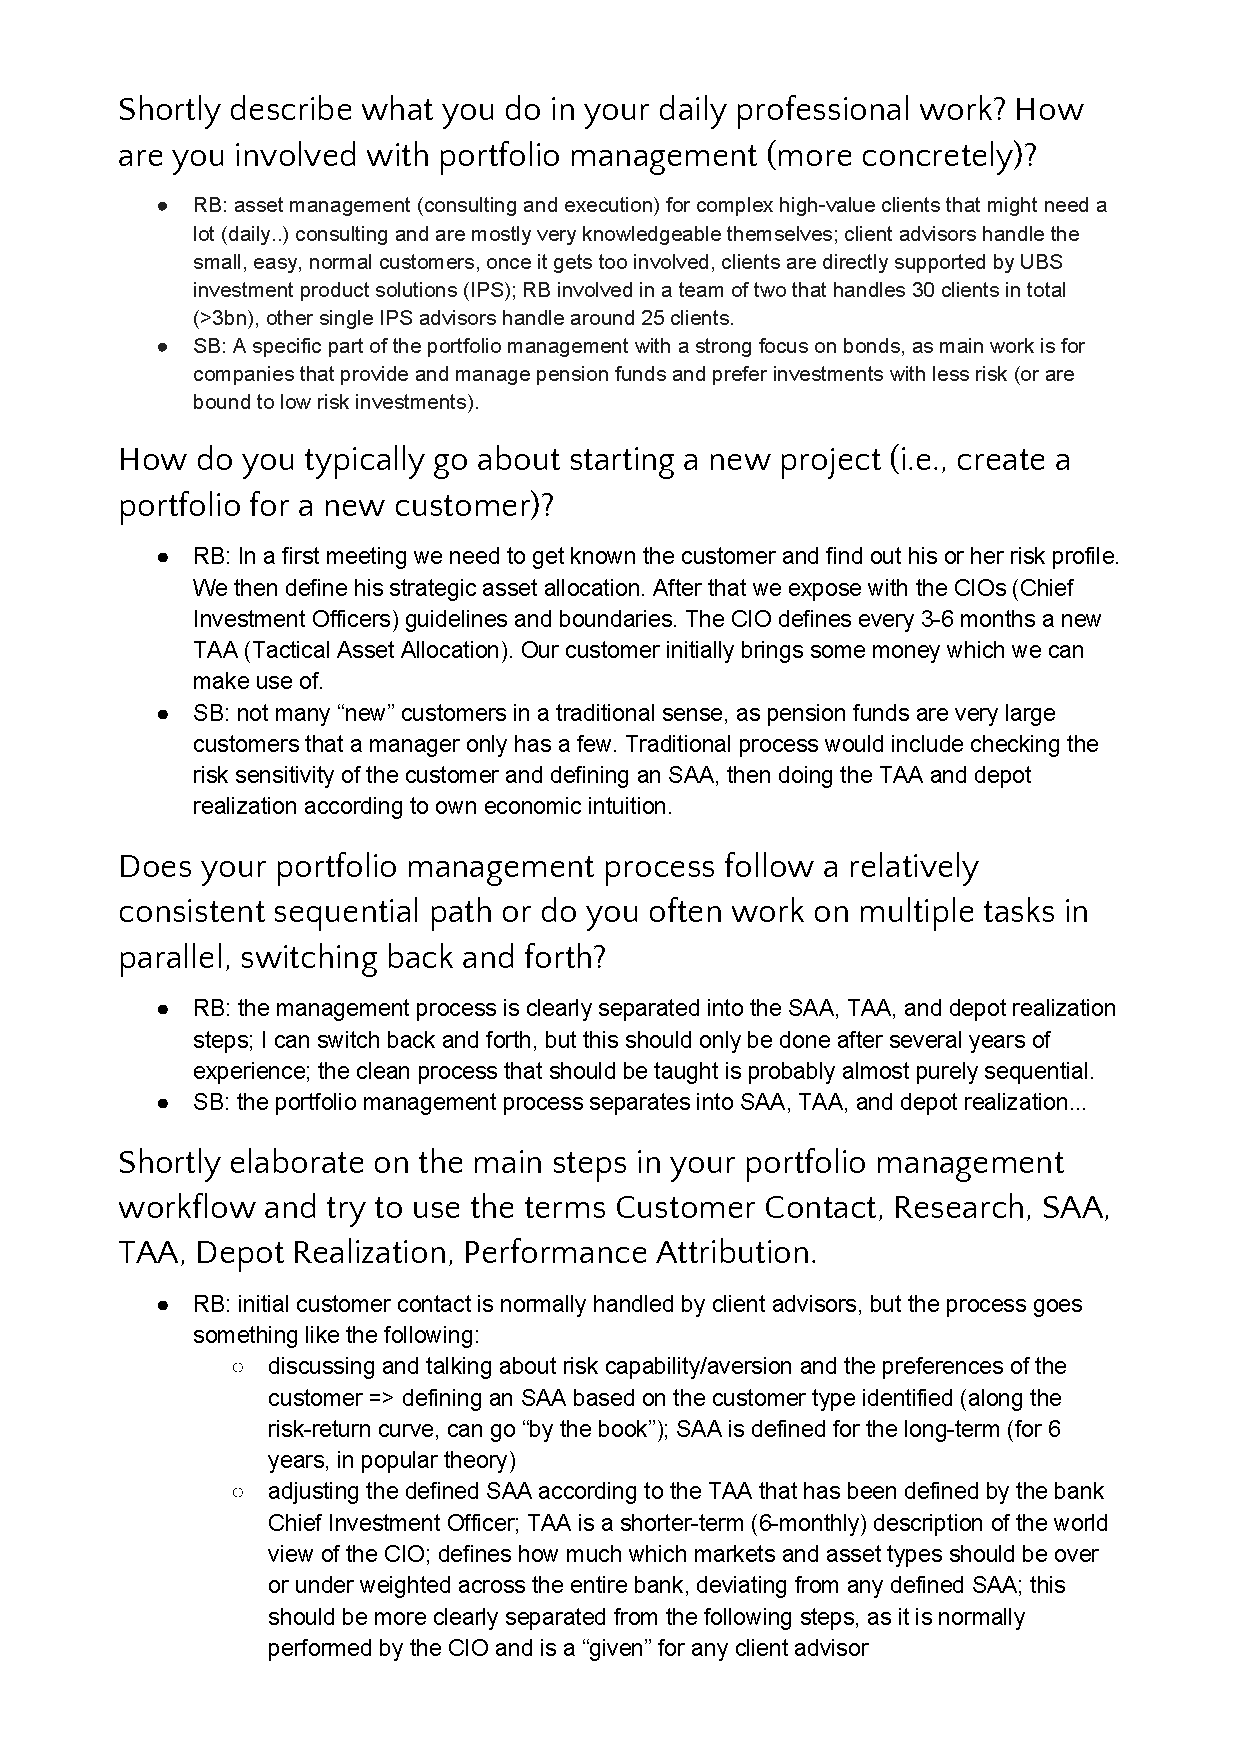
\includepdf[pages={-}, delta=0 20]{appendix/meeting_notes.pdf}
